\section{Reduction to Mixed Integer Linear Programming (MILP)}\label{chap:MILP}

In this chapter, we present how we can reduce the verification problem (Equation (\ref{equ:verification})) to the mixed integer linear programming (MILP) problems, so that it can be solved with the off-the-shelf MILP solvers. We will also consider the over-approximation of the problem so that it is able to be solved with linear programming. We will focus on the ReLU neural network (i.e., all activation functions are ReLU) and the robustness property.

\subsection{Reduction to MILP}

Let $\textbf{x}_c$ be the original input whose label is $y_c=\hat{f}(\textbf{x}_c)$. Recall from Chapter~\ref{sec:robusntessproperty} that, we assume the network $f$ has $K$ layers. Then, Equation (\ref{equ:verification}) can be rewritten as 
\begin{equation}\label{equ:robustnessreduction}
\begin{array}{rll}
  \displaystyle\max_{\textbf{x}}  &   ||\textbf{x} - \textbf{x}_c||_p & \\
    s.t. &  \textbf{x} = \textbf{v}_1, & \\
    & \textbf{up}_{i+1} =  \textbf{W}_i \vec{v}_{i} + \vec{b}_i, & i = 1..K-1\\
    & \textbf{v}_{i+1} = ReLU(\textbf{up}_{i+1}),  & i = 1..K-2 \\
    &  \textbf{up}_{K}(y_c) - \textbf{up}_{K}(y)\geq 0,  & y\in C \\
\end{array}
\end{equation}
where $\textbf{up}_{i},\textbf{v}_{i}$ denote the activation vector of layer $i$ before and after the ReLU function, respectively. 
The first condition confirms to have $\textbf{x}$ as the activation vector of the input layer. 
The second and third conditions implement the linear transformation and ReLU activation function of layer $i+1$, respectively. The fourth condition requires that $\textbf{x}$ has the label $y_c$.  Specifically, the label is $y_c$ if and and only if $\forall {y\in C}:  \textbf{up}_{K}(y_c) - \textbf{up}_{K}(y)\geq 0$. 


%Therefore, if Equation (\ref{equ:robustnessreduction}) returns a value $p^*\geq 0$ then we can conclude that the network $f$ is robust in the neighbourhood $\eta(\textbf{x}_c,L_p,d)$. 

Considering that the ReLU function is non-linear, we introduce two methods of transforming the second and third conditions of Equation (\ref{equ:robustnessreduction}) into MILP constraints, i.e., linear constraints with Boolean variables. 

\subsection*{Method One for Layers}

The first method requires one Binary variable for each neuron. Let $\vec{t}_{i+1}$ have value $0$ or $1$ in its entries and have the same dimension as $\vec{v}_{i+1}$, and $M$ be a very large constant number that can be treated as $\infty$. We do not need $\vec{u}_{i+1}$. Specifically, we have 
the following MILP constraints for every layer $i=1..K-2$ to replace the second and third conditions of Equation (\ref{equ:robustnessreduction}): 
%\begin{align*}
\begin{equation}\label{equ:MILPmethodone}
    \begin{array}{ll}
    \vec{v}_{i+1} &\ge \textbf{W}_i \vec{v}_i + \vec{b}_i,  \\
    \vec{v}_{i+1} &\le \textbf{W}_i \vec{v}_i + \vec{b}_i + M\vec{t}_{i+1}, \\
    \vec{v}_{i+1} &\ge \textbf{0}, \\
    \vec{v}_{i+1} &\le M(1-\vec{t}_{i+1}),
    \end{array}
\end{equation}
%\end{align*}
To understand how it works, if $\vec{t}_{i+1}=\textbf{0}$ then Equation (\ref{equ:MILPmethodone}) can be simplified as $\vec{v}_{i+1}=\textbf{W}_i \vec{v}_i + \vec{b}_i$ and $\textbf{0}\leq \vec{v}_{i+1}\leq M$, which corresponds to the case of $\textbf{up}_{i+1}\geq \textbf{0}$. On the other hand, if $\vec{t}_{i+1}=1$ then Equation (\ref{equ:MILPmethodone}) is reduced to $\vec{v}_{i+1} = \textbf{0}$, which corresponds to the case of $\textbf{up}_{i+1}< \textbf{0}$. These can be extended to work with the general case where the elements in $\vec{t}_{i+1}$ can be either 0 or 1. In such case, the inequalities in Equation (\ref{equ:MILPmethodone}) can be dealt with in an element-wise way. 

Further, if we have additional upper and lower bounds, $\vec{lo}_i$ and $\vec{up}_i$, for $\vec{v}_i$, then Equation (\ref{equ:robustnessreduction}) can be rewritten into 
\begin{equation}\label{equ:equ:MILPmethodtwo}
    \begin{array}{ll}
    \vec{v}_{i+1} &\ge \textbf{W}_i \vec{v}_i + \vec{b}_i,  \\
    \vec{v}_{i+1} & \le \textbf{W}_i \vec{v}_i + \vec{b}_i - \vec{lo}_{i+1}\vec{t}_{i+1}, \\
    \vec{v}_{i+1} &\ge \textbf{0}, \\
    \vec{v}_{i+1} & \le \vec{up}_{i+1}(1-\vec{t}_{i+1}),
    \end{array}
\end{equation}
Note that, the only differences with Equation (\ref{equ:MILPmethodone}) are on the second and fourth conditions, where $\vec{lo}_{i+1}$ and $\vec{up}_{i+1}$ instead of the large number $M$ are used. To understand how it works, if $\vec{t}_{i+1}=\textbf{0}$ then Equation (\ref{equ:equ:MILPmethodtwo}) is reduced to $\vec{v}_{i+1}=\textbf{W}_i \vec{v}_i + \vec{b}_i$ and $\textbf{0}\leq \vec{v}_{i+1}\leq \vec{up}_{i+1}$, which corresponds to the case of $\textbf{up}_{i+1}\geq \textbf{0}$. On the other hand, if $\vec{t}_{i+1}=1$ then Equation (\ref{equ:equ:MILPmethodtwo}) is reduced to $\vec{v}_{i+1} = \textbf{0}$ and $\textbf{W}_i \vec{v}_i + \vec{b}_i \le \vec{v}_{i+1}\le \textbf{W}_i \vec{v}_i + \vec{b}_i - \vec{lo}_{i+1}$. Note that, $\textbf{W}_i \vec{v}_i + \vec{b}_i - \vec{lo}_{i+1}>\textbf{0}$. Therefore, this corresponds to the case of $\textbf{up}_{i+1}< \textbf{0}$. Similarly, Equation (\ref{equ:MILPmethodone}) should be treated in the element-wise way. One of the approaches of computing lower and upper bounds can be seen from Section~\ref{sec:lowupperbounds}.  

\subsection*{Method Two  for Layers} 

Different from the first method, the second method focuses on the ReLU activation function. It requires both $\vec{u}_{i+1}$ and $\vec{v}_{i+1}$.
Specifically, we have 
\begin{equation}\label{equ:methodtwo}
    \begin{array}{ll}
    \vec{u}_{i+1} & = \textbf{W}_i \vec{v}_i + \vec{b}_i,  \\
    \vec{v}_{i+1} & \geq \textbf{0} \\
    \vec{v}_{i+1} & \geq \vec{u}_{i+1} \\
    \vec{v}_{i+1} & \leq \vec{up}_{i+1} \odot \vec{t}_{i+1} \\
    \vec{v}_{i+1} & \leq \vec{u}_{i+1} - \vec{lo}_{i+1} \odot (\textbf{1}-\vec{t}_{i+1}) \\
    \end{array}
\end{equation}
where $\odot$ is the element-wise multiplication. 
To understand how it works, if $\vec{t}_{i+1}=1$ then we have $\textbf{0}  \leq \vec{v}_{i+1}=\vec{u}_{i+1} \leq \vec{up}_{i+1}$, which corresponds to the case of $\textbf{up}_{i+1}\geq \textbf{0}$. On the other hand, if $\vec{t}_{i+1}=\textbf{0}$, then we have $\vec{u}_{i+1} \leq \vec{v}_{i+1}=\textbf{0} \leq  \vec{u}_{i+1} - \vec{lo}_{i+1}$, which corresponds to the case of $\textbf{up}_{i+1}< \textbf{0}$. 


\subsection*{Optimisation Objective}

For the optimisation objective $||\textbf{x} - \textbf{x}_c||_p $ in Equation (\ref{equ:robustnessreduction}),  different conversions are needed for different norm distance metric $L_p$. 

For $L_1$ norm, we introduce auxiliary variables $\textbf{z}$, which bound the absolute value of $\textbf{x} - \textbf{x}_c$, i.e., let $\textbf{z} \leq \textbf{x}_c - \textbf{x}$ and $\textbf{z} \leq \textbf{x} - \textbf{x}_c$. Therefore, we have 
\begin{equation}
\begin{array}{rll}
  \displaystyle\max_{\textbf{x}}  &   \displaystyle  \sum \textbf{z} & \\
    s.t. &  \textbf{x} = \textbf{v}_1, & \\
    & \textbf{up}_{i+1} =  \textbf{W}_i \vec{v}_{i} + \vec{b}_i, & i = 1..K-1\\
    & \textbf{v}_{i+1} = ReLU(\textbf{up}_{i+1}),  & i = 1..K-2 \\
    &  \textbf{up}_{K}(y_c) - \textbf{up}_{K}(y)\geq 0,  & y\in C \\
    & \textbf{z} \leq \textbf{x}_c - \textbf{x} & \\
    & \textbf{z} \leq \textbf{x} - \textbf{x}_c & \\
\end{array}
\end{equation}
where $\sum \textbf{z}$ is the element-wise summation of the vector $\textbf{z}$. 
Note that $\textbf{z}<\textbf{0}$. Therefore, the maximisation over $\sum \textbf{z}$ is to find the closest $\textbf{x}$ (with respect to $\textbf{x}_c$ and $L_1$ norm).  

For $L_\infty$ norm, we introduce a single auxiliary variables $z_\infty$, which bound the $L_\infty$ norm of $\textbf{x} - \textbf{x}_c$, i.e., let $z_\infty \leq \textbf{x}_c(i) - \textbf{x}(i)$ and $z_\infty \leq \textbf{x}(i) - \textbf{x}_c (i)$, for all $i\in [1..s_1]$. Therefore, we have 
\begin{equation}
\begin{array}{rll}
  \displaystyle\max_{\textbf{x}}  &   \displaystyle  z_\infty & \\
    s.t. &  \textbf{x} = \textbf{v}_1, & \\
    & \textbf{up}_{i+1} =  \textbf{W}_i \vec{v}_{i} + \vec{b}_i, & i = 1..K-1\\
    & \textbf{v}_{i+1} = ReLU(\textbf{up}_{i+1}),  & i = 1..K-2 \\
    &  \textbf{up}_{K}(y_c) - \textbf{up}_{K}(y)\geq 0,  & y\in C \\
    & z_\infty \leq \textbf{x}_c(i) - \textbf{x}(i), & i\in [1..s_1] \\
    & z_\infty \leq \textbf{x}(i) - \textbf{x}_c (i), & i\in [1..s_1] \\
\end{array}
\end{equation}
Note that $z_\infty\leq 0$. Therefore, the maximisation over $z_\infty$ is to find the closest $\textbf{x}$ (with respect to $\textbf{x}_c$ and $L_\infty$). 

For $L_2$ norm, the objective becomes quadratic, and therefore we may have to use mixed integer quadratic programming (MIQP), without the need of auxiliary variable. That is, 
\begin{equation}
\begin{array}{rll}
  \displaystyle\max_{\textbf{x}}  &   \displaystyle  \sum_{i=1}^{s_1} (\textbf{x}(i)-\textbf{x}_c(i))^2 & \\
    s.t. &  \textbf{x} = \textbf{v}_1, & \\
    & \textbf{up}_{i+1} =  \textbf{W}_i \vec{v}_{i} + \vec{b}_i, & i = 1..K-1\\
    & \textbf{v}_{i+1} = ReLU(\textbf{up}_{i+1}),  & i = 1..K-2 \\
    &  \textbf{up}_{K}(y_c) - \textbf{up}_{K}(y)\geq 0,  & y\in C \\
\end{array}
\end{equation}


\subsection{Over-approximation with Linear Programming}

Equation (\ref{equ:methodtwo}) can be over-approximated with the below method (illustrated in Figure~\ref{fig:ReLUApprox}) on the ReLU activation function. 
%
\begin{figure}[!htbp]
    \centering
    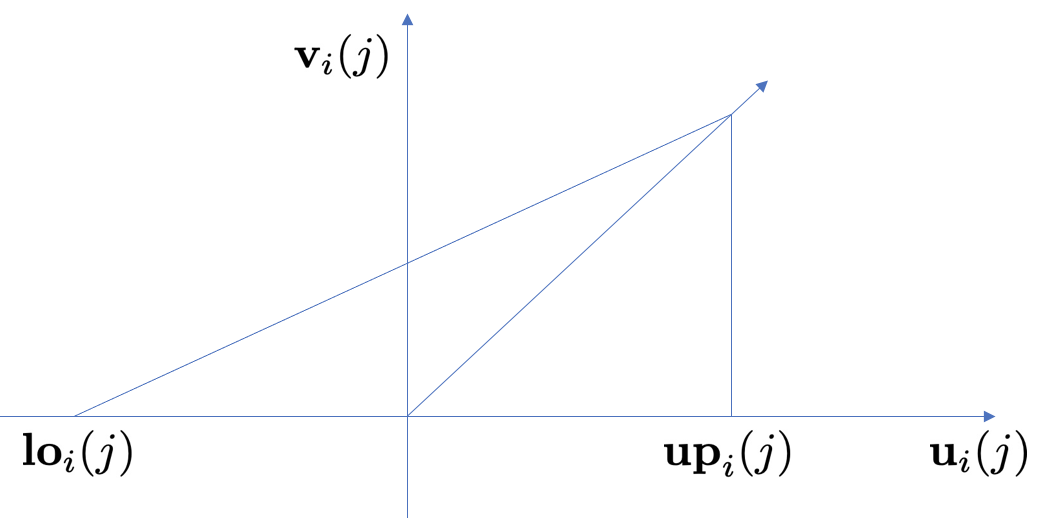
\includegraphics[width=0.7\textwidth]{images/robustnessVerification/ReLUAppro.png}
    \caption{Relaxation of ReLU Activation}
    \label{fig:ReLUApprox}
\end{figure}
Intuitively, when mapping from $\textbf{up}_i(j)$ to $\textbf{v}_i(j)$, instead of using the two lines from ReLU function, i.e., from $(\textbf{lo}_i(j),0)$ to $(0,0)$ and from $(0,0)$ to $(\textbf{up}_i(j),\textbf{up}_i(j))$, we can use the line from $(\textbf{lo}_i(j),0)$ to $(\textbf{up}_i(j),\textbf{up}_i(j))$ to over-approximate the value of $\textbf{v}_i(j)$.  
With this idea, the last three conditions of Equation (\ref{equ:methodtwo}) can be replaced with the below ones for every $j\in [1..s_i]$: 
\begin{equation}\label{equ:MILPapprox}
   \left \{
    \begin{array}{ll}
    \textbf{v}_{i+1}(j)  = 0 & \text{ if } \textbf{up}_{i+1}(j) \leq 0\\
    \textbf{v}_{i+1}(j)  = \textbf{up}_{i+1}(j) & \text{ if } \textbf{lo}_{i+1}(j) \geq 0\\
    \textbf{v}_{i+1}(j)  \geq  0, \textbf{v}_{i+1}(j)  \geq \textbf{up}_{i+1}(j), & \multirow{2}{*}{\text{ otherwise }}\\
    \displaystyle \textbf{v}_{i+1}(j) \leq \frac{\textbf{up}_{i+1}(j)(\textbf{up}_{i+1}(j) - \textbf{lo}_{i+1}(j))}{\textbf{up}_{i+1}(j) - \textbf{lo}_{i+1}(j)} & 
    \end{array}
    \right.
\end{equation}
where the three conditions for the case when $\textbf{up}_{i+1}(j) \geq 0$ and $\textbf{lo}_{i+1}(j) \leq 0$ represent the triangle determined by the three lines such that the value of $\textbf{up}_{i+1}(j)$ will be in the triangle. Therefore, according to the known upper and lower bounds $\textbf{up}_{i+1}(j)$ and $\textbf{lo}_{i+1}(j)$, one of the options in Equation (\ref{equ:MILPapprox})  will be chosen. Note that, all options are linear, without using  any Binary variables. 

Based on the above discussion, if all ReLU activation functions are approximated with Equation (\ref{equ:MILPapprox}), the MILP problem becomes linear programming (LP), which can, in turn, be solved with an LP solver in linear time. We remark that, by approximating the MILP problem (whose computational complexity is NP-complete) with an LP problem (whose computational complexity is in P), solving the optimisation problem becomes tractable, so it is possible to work with a neural network of larger size. 
On the other hand, due to the over-approximation, when we are not able to affirm $d\leq \delta$ as the verification result (as we discussed after Equation (\ref{equ:verification})), we are not able to draw a conclusion on the verification. 

%it is possible that the verification will not return a result when the optimisation problem fails to find a solution.  


\subsection{Computation of Lower and Upper Bounds through Lipschitz Approximation}\label{sec:lowupperbounds}

In this section, we consider how to approximate Lipschitz constant and how to utilise Lipschitz constant for the computation of lower and upper bounds $\textbf{lo}_i$ and $\textbf{up}_i$. Let 
\begin{equation}
    \textbf{G}_i(\textbf{x}) = \displaystyle \frac{\partial \textbf{v}_i}{\partial \textbf{x}} \hspace{1cm}\text{ for } i = 1..K
\end{equation}
be the gradient vector of the hidden activation $\textbf{v}_i$ over the input $\textbf{x}$. 


\subsection*{Approximation of Lipschitz Constant}

We explain how to compute $\textbf{G}_i(\textbf{x})$ by utilising the structural information of the neural network. 
Actually, we will compute both its lower bound $\underline{\textbf{G}}_{i}\in \mathbb{R}^{s_i\times s_1} $ and its upper bound $ \overline{\textbf{G}}_{i}\in \realnumber^{s_i\times s_1}$. 
%
Before proceeding, we define a few notations and operators. Let $[a]_+=\max\{a,0\}$ and $[a]_-=\min\{a,0\}$. For for a matrix $\textbf{F}$, $[\textbf{F}]_+$ and $[\textbf{F}]_-$ are for element-wise max and min. Moreover, we define 
\begin{equation}
    \textbf{W} \otimes [\textbf{lo},\textbf{up}] = [ [\textbf{W}]_+ \times \textbf{lo} + [\textbf{W} ]_- \times \textbf{up}, [\textbf{W}]_+ \times \textbf{up} + [\textbf{W} ]_- \times \textbf{lo}]
\end{equation}
%Moreover, we use $\underline{\textbf{G}}_i\in \realnumber^{s_i\times s_1}$ and $\overline{\textbf{G}}_i\in \real^{s_i\times s_1}$ to denote the lower and upper bound of $\textbf{G}_i$, respectively. 


Actually, we can utilise the chain rule and the sequential structure of the neural network to have the following equation: 
\begin{equation}
    \textbf{G}_i(\textbf{x}) = \frac{\partial \Vec{v}_i}{\partial \Vec{x}} = \frac{\partial \Vec{v}_{i}}{\partial \Vec{u}_{i}}\frac{\partial \Vec{u}_{i}}{\partial \Vec{v}_{i-1}}... \frac{\partial \Vec{v}_{2}}{\partial \Vec{u}_{2}}\frac{\partial \Vec{u}_{2}}{\partial \Vec{v}_{1}}
\end{equation}
which suggests that the gradient $\textbf{G}_i(\textbf{x})$ can be computed repeatedly over the layers. Note that, $\displaystyle\frac{\partial \Vec{u}_{i}}{\partial \Vec{v}_{i-1}}=\textbf{W}_{i-1}$, where $\textbf{W}_{i-1}$ is the weight matrix of layer $i-1$.
Let $\nabla\Vec{\sigma}_i = \displaystyle\frac{\partial \Vec{v}_{i}}{\partial \Vec{u}_{i}}\in \real^{s_{i}\times s_i}$, we have 
\begin{equation}
\textbf{G}_i(\textbf{x}) = \frac{\partial \Vec{v}_i}{\partial \Vec{x}} = \nabla\Vec{\sigma}_{i}\textbf{W}_{i-1}...\textbf{W}_2\nabla\Vec{\sigma}_2\textbf{W}_1
\end{equation}
Let ${\underline{\Lambda}}_i,{\overline{\Lambda}}_i\in \real^{s_i\times s_i}$ be the diagonal matrices denoting the lower and upper bound of $\nabla\Vec{\sigma}_i$, respectively. For ReLU activation function, we have 
\begin{equation}
   \textbf{1} \geq {\overline{\Lambda}}_i\geq {\underline{\Lambda}}_i\geq \textbf{0} 
\end{equation}



To enable a computation of the lower and upper bounds, we use an iterative process as follows. Let $\textbf{F}_{i+1}=\textbf{W}_i\textbf{G}_i$ (i.e., $=\displaystyle\frac{\partial \Vec{u}_{i+1}}{\partial \Vec{x}}$), we have \begin{equation}
    \textbf{G}_i = \nabla\Vec{\sigma}_i\textbf{F}_i = \nabla\Vec{\sigma}_i\textbf{W}_{i-1}\textbf{G}_{i-1}
\end{equation}
The computation proceeds as follows. Initially, we have 
\begin{equation}
    \underline{\textbf{G}}_0 = \overline{\textbf{G}}_0 = \textbf{I}
\end{equation}
where $\textbf{I}$ is the identify matrix. Then, given $\underline{\textbf{G}}_{i-1} $ and $ \overline{\textbf{G}}_{i-1}$, we have 
\begin{equation}
\begin{array}{rll}
    [\underline{\textbf{F}}_{i},\overline{\textbf{F}}_{i}] =  &  \textbf{W}_i \otimes [\underline{\textbf{G}}_{i-1}, \overline{\textbf{G}}_{i-1}] & \\
    \overline{\textbf{G}}_i = & \max \{\underline{\Lambda}_i\overline{\textbf{F}}_i,\overline{\Lambda}_i\overline{\textbf{F}}_i\} = & \overline{\Lambda}_i[\overline{\textbf{F}}_i]_++\underline{\Lambda}_i[\overline{\textbf{F}}_i]_-\\
    \underline{\textbf{G}}_i = & \min \{\underline{\Lambda}_i\underline{\textbf{F}}_i,\overline{\Lambda}_i\underline{\textbf{F}}_i\} = & \underline{\Lambda}_i[\underline{\textbf{F}}_i]_++\overline{\Lambda}_i[\underline{\textbf{F}}_i]_- \\
\end{array}
\end{equation}

Finally, given an input region, which can be either the entire input domain or a $d$-neighbourhood, if we know ${\overline{\Lambda}}_i$ and ${\underline{\Lambda}}_i$, we can compute $[\underline{\textbf{G}}_i, \overline{\textbf{G}}_i]$ with respect to the input region. Therefore, this method can be used to compute either the global Lipschitz constant (when the input region is the entire input domain) or the local Lipschitz constant  (when the input region is a $d$-neighbourhood). 

\subsection*{Computation of Lower and Upper Bounds}

Let $\eta(\textbf{x},L_p,d)$ be a $d$-neighbourhood centred around $\textbf{x}$, we can first use the above method to compute $[\underline{\textbf{G}}_i, \overline{\textbf{G}}_i]$. 
Then,  the upper bound and lower bounds of the $j$-th dimension are as follows: 
\begin{equation}
\begin{array}{cc}
    \textbf{up}_i(j) = & \textbf{v}_i(j) +  \overline{\textbf{G}}_i(j)  \max_{\textbf{x}'\in \eta(\textbf{x},L_p,d)} |\textbf{x}(j) - \textbf{x}'(j)|  \\
    \textbf{lo}_i(j) = & \textbf{v}_i(j) - \underline{ \textbf{G}}_i(j)  \max_{\textbf{x}'\in \eta(\textbf{x},L_p,d)} |\textbf{x}(j) - \textbf{x}'(j)|\\
\end{array}
\end{equation}

